\documentclass[12pt, letterpaper]{article}
%\documentclass[12pt, letterpaper]{amsart}

%%%%%%%%%%%% LANGUAGE & ENCODING %%%%%%%%%%%%%%%%%
\usepackage[english]{babel}
\usepackage[utf8]{inputenc}%%%% to process umlauts and accents directly
%\usepackage{indentfirst}
%\usepackage{ucs}

%%%%%%%%%%% PACKAGES %%%%%%%%%%%%%%%%%%%%%%%%%%%%%
% For Hyperlinks
\usepackage[colorlinks,linkcolor=cyan,citecolor=magenta]{hyperref}

% Common math packages
\usepackage{amsthm, amsmath, amsfonts, amssymb, esint, mathrsfs, mathtools}
\usepackage{tensor} % To handle multi-index notation
\usepackage[capitalize,nameinlink]{cleveref} % Nice references
\crefname{equation}{}{} % Removes Eq. from equation references
\numberwithin{equation}{section} % Number equations within each section separately

% Extra symbols
\usepackage{stmaryrd} % contains \owedge  for Kulkarni-Nomizu product and some other special characters
\usepackage{commath} % contains \norm \abs

% Some useful packages
\usepackage{verbatim} %%% enables \begin{comment}    \end{comment}
\usepackage{enumerate} % allows different types of indices
\usepackage{float} % Handling figures

%%%%%%%%%%% MARGINS %%%%%%%%%%%%%%%%%%%%%%%%%%%%%%%%
% Margins
\usepackage[top=1in, bottom=1in, left=1in, right=1in]{geometry}

%%%%%%%%%%% CUSTOM NOTATION  %%%%%%%%%%%%%%%%%%%%%%
\newcommand{\N}{\mathbb{N}}
\newcommand{\Z}{\mathbb{Z}}
\newcommand{\Q}{\mathbb{Q}}
\newcommand{\R}{\mathbb{R}}
\newcommand{\C}{\mathbb{C}}
\newcommand{\K}{\mathbb{K}}

\newcommand{\f}{\mathfrak}
\newcommand{\ul}{\underline}
\newcommand{\mb}{\mathbb}
\newcommand{\mr}{\mathrm}
\newcommand{\mf}{\mathbf}
\newcommand{\mc}{\mathcal}
\newcommand{\e}{\emph}
\newcommand{\vp}{\varphi}
\newcommand{\ve}{\varepsilon}

\newcommand{\vol}{\operatorname{Vol}}
\newcommand{\diam}{\operatorname{diam}}
\newcommand{\dist}{\operatorname{dist}}
\newcommand{\dv}{\operatorname{div}}
\newcommand{\tr}{\operatorname{tr}}

\newcommand{\dd}{\; \mathrm{d}} %%%% d for integration dx
\newcommand{\wt}{\widetilde}
\newcommand{\ol}{\overline}

%%%%%%%%%%% THEOREMS %%%%%%%%%%%%%%%%%%%%%%%%
\newtheorem{theorem}{Theorem}[section]
\newtheorem{lemma}[theorem]{Lemma}
\newtheorem{proposition}[theorem]{Proposition}
\newtheorem{conjecture}[theorem]{Conjecture}
\newtheorem{corollary}[theorem]{Corollary}
\newtheorem{claim}[theorem]{Claim}
\newtheorem{problem}[theorem]{Problem}
\newtheorem{remark}[theorem]{Remark}

\theoremstyle{definition}
\newtheorem{definition}[theorem]{Definition}

\theoremstyle{remark}
\newtheorem{example}[theorem]{Example}


%%%%%%%%%%% TITLE %%%%%%%%%%%%%%%%%%%
%\title[CIS625: Computational Learning Theory]{Computational Learning Theory Lecture Notes}
%\author[Notes by Martin Citoler-Saumell]{Martin Citoler-Saumell}
%\date{Spring 2017}
%\address{University of Pennsylvania\\ Philadelphia, PA 19104}
%\email{\href{mailto:martinci@math.upenn.edu}{martinci@math.upenn.edu}}

\title{Computational Learning Theory Lecture Notes}
\author{Martin Citoler-Saumell}
\date{CIS625 Spring 2017}

%%%%%%%%%%% DOCUMENT BEGINS %%%%%%%%%%%%
\begin{document}

%------------------------------------------------------------
%          LECTURE 2
%------------------------------------------------------------
\section{Lecture 2: 2017.01.30}

\begin{remark}[PAC Learning]
    Fixing the class $\mc C$ is a strong assumption, it is the prior you are assuming about the true behavior of the data.
     For example, when you fit a linear regression, you are assuming that there is a true linear relation in the data.
    
    In contrast, the assumption on the distribution over $X$ is fairly general.
\end{remark}

\begin{theorem}
    The class of rectangles over $\R^2$ from example above is PAC learnable (with sample size $m\sim\frac1\ve\ln\left(\frac1\delta\right)$).
\end{theorem}

\subsection{PAC learning boolean conjunctions}

In the following we are going to see an example of problem that is PAC learnable.
\begin{itemize}
    \item $X = \lbrace 0, 1 \rbrace^n$
    \item Class $\mc C = $ all conjunctions over $x_1,\ldots,x_n$. $\abs{\mc C} = 3^n$\\
          E.g.: If $c = x_1\wedge \lnot x_3 \wedge \lnot x_{11} \wedge x_{26} \ldots$,
          \begin{align}
              c(\vec x) = 1 \iff x_1 =1, x_3 = 0, x_{11} = 0, x_{26} = 1, \ldots
          \end{align}
    \item $D$ over $\lbrace 0, 1 \rbrace^n$.
\end{itemize}


\subsubsection[Algorithm for monotone case]{Algorithm for monotone case (i.e. no $\lnot$'s)}

In this case we are trying to fit something like $c = x_1\wedge x_5 \wedge x_{13} \ldots$. i.e. given some examples of sequences of bits and the result of $c$ on them, we are trying to guess what the conjunction $c$ actually is.
We can use the following algorithm:
\begin{itemize}
    \item $h \leftarrow x_1\wedge x_2 \wedge x_3\wedge \ldots \wedge x_n$, start with the conjunction of all the variables.
    \item For each positive example, $\langle \vec x, 1 \rangle$, delete any variable in $h$ such that $x_i=0$.\\
    This method ensures that the positives of $h$ is a subset of the true $c$.
\end{itemize}


\subsubsection*{Analysis}

Let $p_i$ denote the probability we delete $x_i$ from $h$ in a single draw. In other words,
\begin{align}
    p_i = \mb P_{\bar X\sim D}[c(\vec x) = 1, x_i=0].
\end{align}
Then we have an a priori bound on error: $Err(h) \leq \sum\limits_{x_i\in h} p_i$.
 We can make a distinction between \emph{bad} and \emph{good} indices. 
 An index, $i$, is bad if $p_i\geq \frac{\ve}{n}$ and good otherwise. 
 Note that if $h$ contains no bad indices, then we have
\begin{align}
    Err(h) \leq \sum\limits_{x_i\in h} p_i \leq n\left(\frac{\ve}{n}\right).
\end{align}
Let's fix some index, $i$, such that $p_i\geq \frac\ve n$. i.e. a bad index. We have that
\begin{align}
    \mb P[x_i\textrm{ "survives" m random samples}] &= (1 - p_i)^m \quad (iid)\\
    & \leq \left(1 - \frac\ve n\right)^m \\
    \mb P[\textrm{\emph{any} bad i "survives" m random samples}] &\leq n\left(1 - \frac\ve n\right)^m.
\end{align}
If we want the right-hand-side of the last inequality to be less than some $\delta>0$, we end up with $m \geq \frac n\ve \ln\left(\frac n\delta\right)$. 
In other words, we just proved the following theorem

\begin{theorem}
    Conjunctions over $\lbrace 0,1 \rbrace^n$ are PAC learnable with sample size  $m \geq \frac n\ve \ln\left(\frac n\delta\right)$.
\end{theorem}

\begin{remark}
    An analogous argument proves this theorem for conjunctions that are not necessarily monotone. 
    The only difference is that we have to keep track the extra $\lnot$ variables.
\end{remark}

\begin{remark}
    We can identify some pattern for this kind of analysis. 
    We identify some ``bad'' things that may happen and then prove that the probability of them happening decreases fast when we increase the number of samples seen.
\end{remark}


\subsection{Hardness of PAC learning 3-term DNF}

Now we are going to see an example of non PAC learnable problem. 
However, we will be able to slightly modify it and achieve PAC learning. 
This motivates an better definition of PAC learnable.
\begin{itemize}
    \item Input space $X = \lbrace 0, 1 \rbrace^n$
    \item Class $\mc C = $ all disjunctions of three conjunctions. $\abs{\mc C} = 3^{3n}$\\
          E.g.: If $c = T_1 \lor T_2 \lor T_3$ where $T_i$ is a conjunction over $X$.\\
          $c = \left(x_1 \wedge x_7 \wedge \lnot x_8 \right) \lor \left(x_2 \wedge x_5 \wedge \lnot x_7 \wedge \lnot x_8\right) \lor \left(x_6 \wedge x_{12}\right)$.
\end{itemize}
To see that this problem is \emph{hard}, we prove that the graph 3-coloring problem reduces to the 3-term DNF problem. 

\subsubsection*{Graph 3-coloring to PAC learning 3-term DNF}

Suppose that you have a 3-colorable (undirected) graph $G$. 
That is, a graph such that we can color the vertices with 3 colors in such a way that there are no edges between vertices of the same color. 
We see an example of how to transform such a graph into a set of labeled examples for the PAC learning 3-term DNF. 
\begin{figure}[H]
\centering
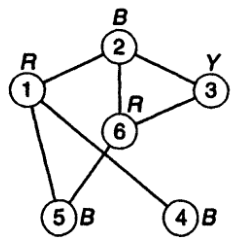
\includegraphics[width=0.3\linewidth]{../img/graph}
\caption{A graph with a 3-coloring.}
\label{fig:graph}
\end{figure}
First, for the $i$-th node we create a positive example that is represented by the vector, $v(i)$, with a 0 in the $i$-th entry and 1's everywhere else. E.g. from node one we have $\langle 011111, + \rangle$.
Then we create a negative example from each edge that is represented by a vector, $e(i,j)$, of 1's except for 0's at the positions that determine the edge. 
E.g. from the edge connecting 2 and 3 we obtain $\langle 100111, - \rangle$.
Next, the coloring can be used to define a 3-term DNF in the following way. 
Given a color, we define $T_{color}$ as the conjunction of the variables/vertices that are \emph{not} of that color. In this example we have
\begin{align}
    T_R = x_2 \wedge x_3 \wedge x_4 \wedge x_5,\\
    T_B = x_1 \wedge x_3 \wedge x_6,\\
    T_Y = x_1 \wedge x_2 \wedge x_4 \land x_5 \land x_6 .
\end{align}

\begin{claim}
    $G$ is 3-colorable $\iff$ there is a 3-term DNF \emph{consistent} with the labeled sample above.
\end{claim}
\begin{proof}
    We have just seen how to obtain a 3-term DNF from a 3-colorable graph. We only need to check that it is consistent with the sample. 
    By construction, all the positive examples satisfy $T_{color}$ where color is the vertex's color, since the only 0 in the vector is in the position that is dropped. 
    Similarly, it follows that the examples coming from the edges do not satisfy any of the $T$'s. In any edge there are two colors corresponding to its vertices. 
    The extra 0 in the example ensures that the $T$'s from those colors are not satisfied.
    Finally, the $T$ of the remaining color cannot be satisfied because both vertices are included in the conjunction and they are both 0 in the example.
    
    Conversely, given a graph and the labeled examples as above, if there is a consistent 3-term DNF we can find a coloring in the following way. 
    Label each term of the formula with a color, say $T_R \lor T_Y \lor T_B$, and remember the order of the labels. 
    Then, we define the color of vertex $i$ (corresponding to vector $1\ldots101\ldots1$) as the label of the first formula that is satisfied by $v(i)$. 
    Since the formula is consistent with the sample, every vertex must be actually colored. We only need to argue that this is a valid coloring. 
    Suppose to the contrary that $i$ and $j$ are to vertices that are connected by an edge and have the same color. 
    This means that both $v(i)$ and $v(j)$ satisfy $T_{C_0}$. 
    However, we also have $v(i) \& v(j) = e(i,j)$  where $\&$ denotes the bit-wise and operation and it follows that $e(i,j)$ satisfies $T_{C_0}$, a contradiction with the consistency of the formula since edges are negative examples.
\end{proof}

This concludes the argument that finding a coloring of a graph is the same as producing a consistent 3-term DNF. 
We are only left with the computational aspects.
Namely, given the labeled sample associated to a graph, we need to find a way to feed it to a PAC learning algorithm. 
First we need a distribution over vectors of bits.
For this we can just sample the examples uniformly. 
Finally, to ensure consistency we choose $\ve$ any quantity less than $\frac1{\#examples}$\footnote{This epsilon is allowed because $\frac1\ve$ is polynomial in the size of input. This is not true in general.}. This way the algorithm cannot make any mistakes is forced to be consistent. The $\delta$ can be arbitrary.
In conclusion, if the 3-term DNF problem were PAC learnable, we could solve the coloring problem in random polynomial time. 
Another way to say this is in the form of the following theorem.
\begin{theorem}
    If 3-term DNF are PAC learnable, then $NP = RP$.
\end{theorem}
Of course, it is strongly believed that $RP \subsetneq NP$ so this is rather strong evidence against the easiness of the 3-term DNF problem.

\begin{remark}
    The upshot is that a slight generalization of the conjunction problem, for which we have a randomized polynomial time solution, is almost assured to not be PAC learnable ( unless NP = RP)
\end{remark}

\end{document}
